%%%
% (PACT) Submit full papers (up to 15 pages) or extended abstracts (5-7 pages) 
%%%


% This is samplepaper.tex, a sample chapter demonstrating the
% LLNCS macro package for Springer Computer Science proceedings;
% Version 2.21 of 2022/01/12
%
\documentclass[runningheads]{llncs}
%
\usepackage[T1]{fontenc}
% T1 fonts will be used to generate the final print and online PDFs,
% so please use T1 fonts in your manuscript whenever possible.
% Other font encondings may result in incorrect characters.
%
\usepackage{verbatim}
\usepackage{graphicx}
\usepackage{subcaption}
\usepackage{hyperref}
\usepackage{listings}
\usepackage{courier}
\usepackage{epstopdf}
\usepackage{textcomp}
\usepackage{minted}
\usepackage{color}

% \lstset{language=[Sharp]C}
\lstset{numbers=left,xleftmargin=3em,numberstyle=\footnotesize\ttfamily,captionpos=b}
\lstset{basicstyle=\footnotesize\ttfamily}
% Used for displaying a sample figure. If possible, figure files should
% be included in EPS format.
%
% If you use the hyperref package, please uncomment the following two lines
% to display URLs in blue roman font according to Springer's eBook style:
%\usepackage{color}
%\renewcommand\UrlFont{\color{blue}\rmfamily}
%\urlstyle{rm}
%
\begin{document}
%
%\title{Brahma.FSharp: Power of Functional Programming to Utilize GPGPU in .NET Applications}
\title{Brahma.FSharp: Power of Functional Programming to Create Portable GPGPU-enabled .NET Applications}
%
\titlerunning{Brahma.FSharp to Create Portable GPGPU-enabled .NET Apps}
% If the paper title is too long for the running head, you can set
% an abbreviated paper title here
%
\author{Nikolai Ponomarev\inst{1}\orcidID{0009-0000-2382-5687} \and
Vladimir Kutuev\inst{1}\orcidID{0000-0001-7749-4940} \and
Semyon Grigorev\inst{1}\orcidID{0000-0002-7966-0698}}
%
\authorrunning{N. Ponomarev, V. Kutuev, S. Grigorev}
% First names are abbreviated in the running head.
% If there are more than two authors, 'et al.' is used.
%
\institute{Saint Petersburg State University, 7-9 Universitetskaya Embankment, St. Petersburg, Russia \and
\email{n.ponomarev@spbu.ru, v.kutuev@spbu.ru, s.v.grigoriev@mail.spbu.ru}}
%
\maketitle              % typeset the header of the contribution
%
\begin{abstract}
Widening of GPGPU applicability increases the interest to high-level languages for GPGPU programming development.
One of the challenges is to create a portable solution which provides static checks and being integrated with application platforms.
We propose a tool---Brahma.FSharp---that allows one to utilize OpenCL-compatible devices in .NET applications, and to develop homogeneous code using familiar .NET tools.
Brahma.FSharp provides ability to create GPU kernels using F\# programming language that is functional-first statically typed .NET language.
Compile-time metaprogramming techniques, provided by F\#, allows one to develop generic type-safe kernels.
We show portability of the proposed solution by running several algorithms developed with it across different platforms and devices.
    
\keywords{Functional programming \and GPGPU  \and FSharp \and .NET \and OpenCL}
\end{abstract}

\section{Introduction}

Last decades utilization of GPGPUs not only in scientific or dedicated applications, but also in regular business applications becomes more popular.
In such cases not peak performance, but transparent offloading of computations to accelerator has come into focus.
As a result, respective tools for integration of GPGPUs into such platforms as JVM~\cite{rootbeer,jcuda,ScalaGPU} or .NET~\cite{FSCLPhD,aleaGPUasync} are developed.
Note that in real-world application the problem no only to offload some computations on GPGPU, but to orchestrate heterogenous asynchronous application that involves computations on possible several GPGPUs.

At the same time, utilization of existing functional languages and creation new ones for GPGPU programming, looks promising due to them safety, flexibility, ability to use advanced optimization techniques and to create high-level abstractions.
That lead to such projects as Futhark~\cite{10.1145/3140587.3062354}, Lift~\cite{10.5555/3049832.3049841}, AnyDSL~\cite{10.1145/3276489}, Accelerate~\cite{10.1145/1926354.1926358}.
 
Nowadays there are very few combination of mature business application development platform and functional programming language.
One of them is a .NET platform and F\# programming language. 
There are several tools, such as Alea.GPU~\cite{aleaGPUasync}, FCSL~\cite{FSCLPhD}, ILGPU~\footnote{ILGPU project web page: \url{https://ilgpu.net/}}, that allows one to integrate GPGPUs into .NET application without using such unsafe and low-level mechanisms like string-level kernels creation. 
While FSCL and Alea.GPU use F\# to create kernels, ILGPU works on IL level that limits ability to use high-level features and nontrivial optimizations.
 
In this work we propose a \textbf{Brahma.FSharp}\footnote{
    Sources of Brahma.FSharp: \url{https://github.com/YaccConstructor/Brahma.FSharp}.
} --- the tool for portable GPGPU-enabled .NET applications development that provides transparent and safe integration with accelerators --- and demonstrate it's portability across variety of platforms and devices. 
%\input{RelatedWork}
\section{Brahma.FSharp}

Brahma.FSharp is a tool that allows one to utilize GPGPUs in .NET applications and write kernels and all supplementary code in pure F\#~\cite{fsharp} that is a functional-first multiparadigmal programming language for .NET platform.
This language combines functional programming, including first-class functions, generics, static strong typing with automatic type inference, with transparent integration with a platform for business applications development with mature infrastructure.
At the same time, F\# provides an ability to write imperative code that is native for kernel programming.

Core of the tool is a translator of F\# subset to OpenCL C that is based on \emph{code quotations}~\cite{FSharpQuotations} that allows one to get access to annotated tree of the F\# code and transform it during program execution.
This tree can be transformed using regular F\# functions: for example, it can be translated to other language, that is we do to generate OpenCL C code for kernels.
Other words, code quotations is a runtime metaprogramming feature that allows us to create kernels configurable during program execution.
For example, in opposite to compile time metaprogramming, it is possible to configure work group size dependent parts of kernel (e.g. local buffer size) without recompilation of whole program (look at line 9 of listing~\ref{lst:mXm_kernels}).
The main feature is that everything is strongly and statically typed: no unsafe code that uses strings, pointers, objects, etc.
At the user side, compiled quotation (compiled kernel) has the signature that requires parameters of types that are in agreement with initial quotation.

An example of quoted code (actually, part of the generalized mXm kernel) is presented in listing~\ref{lst:mXm_kernels} (lines 6--12).
This code also demonstrates typed composition of quotations: operations \verb|opAdd| and \verb|opMult|, and identity element \verb|zero|, have agreed types and can be specified outside the kernel in run time.
So, we can write highly configurable kernels generator and instantiate specific kernels later, as shown in lines 15--16.

\begin{listing}
    \begin{minted}[linenos]{fsharp}
  let mXmKernel    
     (opAdd: Quotations.Expr<'a -> 'b -> 'a>) 
     (opMult: Quotations.Expr<'e -> 'f -> 'b>) 
     (zero: Quotations.Expr<'a>) ... (* other parameters *)  =
        ... // Supplementary code
        let kernel = <@ fun 2dRange m1 m2 res ->  // Quoted code
          ... 
          let acc = %zero // Embedded identity value
          let lBuf = localArray lws // captured from context
          ... 
          acc <- (%opAdd) acc ((%opMult) x y) // Embedded operations
          ... @>
        ... // Supplementary code
    
  let intArithmeticKernel = mXmKernel <@ (+) @> <@ ( * ) @> <@ 0 @>
  let intMinPlusKernel = 
      mXmKernel <@ (min) @> <@ (+) @> <@ Int.MaxValue @>
    \end{minted}
    \caption{An example of generic matrix multiplication kernel}
    \label{lst:mXm_kernels}
  \end{listing}

The translator supports not only imperative subset of F\# and primitive types, but also F\#-specific features like structs, tuples, discriminated unions, pattern matching, nested bindings.
Also it supports OpenCL specific features like atomic functions, barriers, local and thread-local arrays allocation.
For data transferring and manipulation Brahma.FSharp provides \verb|ClArray<'t>| and \verb|ClCell<'t>| primitives that are F\#-array-friendly wrappers for \texttt{ClBuffer}.

Brahma.FSharp provides typical workflow to run kernels and implements respective typed wrappers for it\footnote{Configuration of path to \texttt{libopencl} allows one to make the solution portable.}.
It is worth noting that F\# is friendly to asynchronous programming and provides huge amount of parallel and asynchronous programming primitives~\cite{FSharpAsync}.
Utilization of \emph{MailboxProcessor}, that is F\#-native massage passing primitive, to wrap command queue allows us to make communication with GPGPU friendly for asynchronous programming in F\#.
\section{Evaluation}

In this section we provide experiments\footnote{Sources of benchmarking automation infrastructure: \url{https://github.com/vkutuev/matrix-benchmark}.} with Brahma.FSharp platform which are aimed to demonstrate its main features on regular (not HPC) devices\footnote{Looks more suitable for business applications that use .NET.}. 
We evaluated Brahma.FSharp in two cases listed below and described in respective sections.
\begin{enumerate}
\item The first one is an image convolution that demonstrates utilisation of several GPU-s using F\# MailboxProcessor.
\item Second one is a matrix multiplication that demonstrates ability to create generic strongly statically typed kernels, to utilize local and private memory for performance optimization, and to demonstrate portability across different devices.
\end{enumerate}


\subsection{Image Convolution}

We implement image convolution in order to demonstrate multiple GPGPUs utilization.
Native for F\# asynchronous model, as was shown in~\cite{aleaGPUasync}, simplifies creation of complex workflows that include GPGs.
We use F\# MailboxProcessor because Brahma.FSharp provides it as an interface for communication with GPUs.
Kernel is simply wrapped as shown in~\ref{lst:img_conv}. 
Simple load balancer that send next image to an agent with less number of messages in input queue was implemented.

\begin{listing}[h]
  \begin{minted}[linenos]{fsharp}
let imgProcessor filter (imgSaver: MailboxProcessor<_>) =
    MailboxProcessor.Start(fun inbox ->
        let rec loop ... = async { // Async message processing loop
            let! msg = inbox.Receive() // Load message
            match msg with
            | EOS ch -> // Handle end of stream
                imgSaver.PostAndReply EOS
                ch.Reply()
            | Img img -> // Handle image
                let filtered = filter img // Convolution
                imgSaver.Post (Img filtered)
                return! loop ... }// Got to next message
        loop ...)
  \end{minted}
  \caption{MailboxProcessor-based wrapper for kernel to make it easier to integrate it to complex workflow}
  \label{lst:img_conv}
\end{listing}

We evaluate this solution on a \textbf{Lenovo} platform with two GPUs: NVIDIA GeForce MX150 and Intel(R) UHD Graphics 620.
We assume that all images are loaded into RAM and converted to grayscale. 
Typical chain of filters is applied: 3 gaussian blur ($5 \times 5$ kernel), then edges detection ($5 \times 5$ kernel).
420 images (1gb of data) was handled in 40 seconds with two GPUs, in 64 seconds using Nvidia GPU only, and in 97 seconds using Intel GPU only.
Thus we can see that even naive multi-GPU workflow allows one to achieve up to 30\% speedup.

\subsection{Matrix Multiplication}

We evaluate generic kernel parametrized by types and operations~\ref{lst:mXm_kernels}, implemented in F\#.
Several basic optimizations, inspired by ``Tutorial: OpenCL SGEMM tuning for Kepler'' by Cedric Nugteren\footnote{``Tutorial: OpenCL SGEMM tuning for Kepler'': \url{https://cnugteren.github.io/tutorial/pages/page1.html}}, were applied.
Namely, we use tiling in local and private memory.
But current version supports only square matrices and square tiles.

\begin{figure}
  \begin{center}
  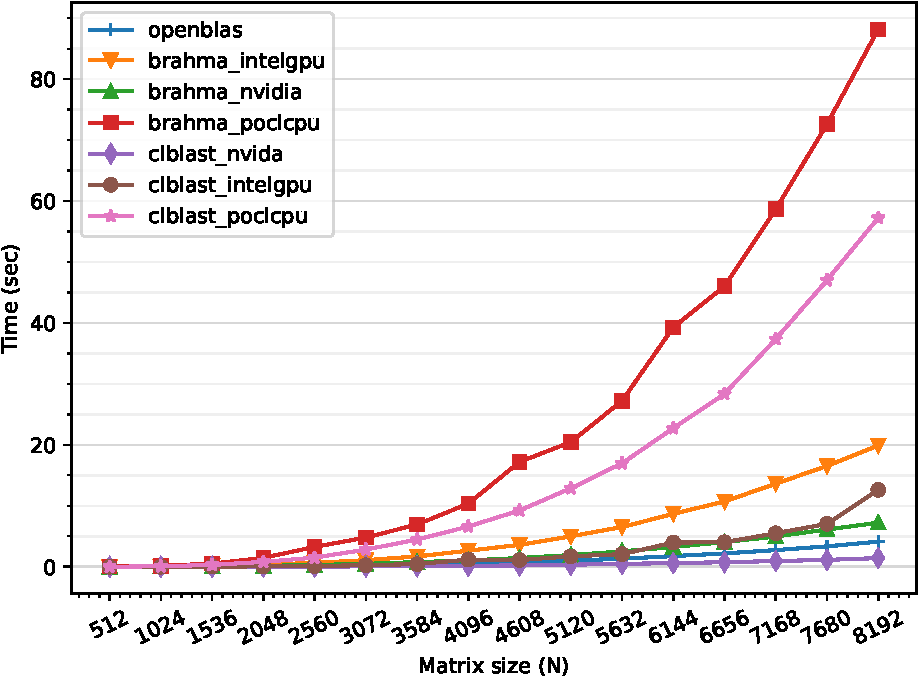
\includegraphics[width=0.45\textwidth]{../data/Lenovo-T480_crop.pdf}
  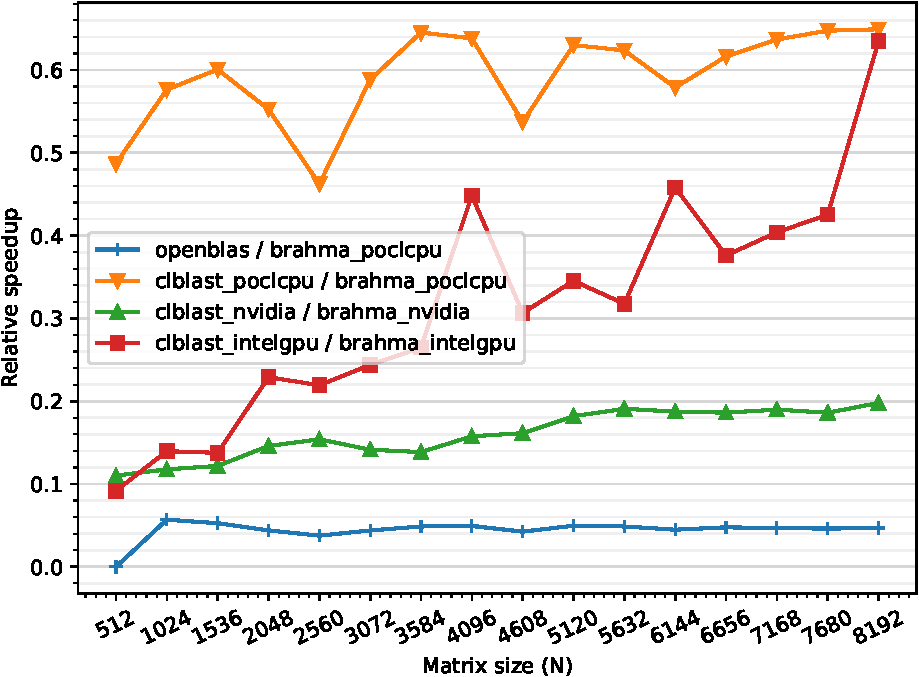
\includegraphics[width=0.45\textwidth]{../data/Lenovo-T480_rel_crop.pdf}\\
  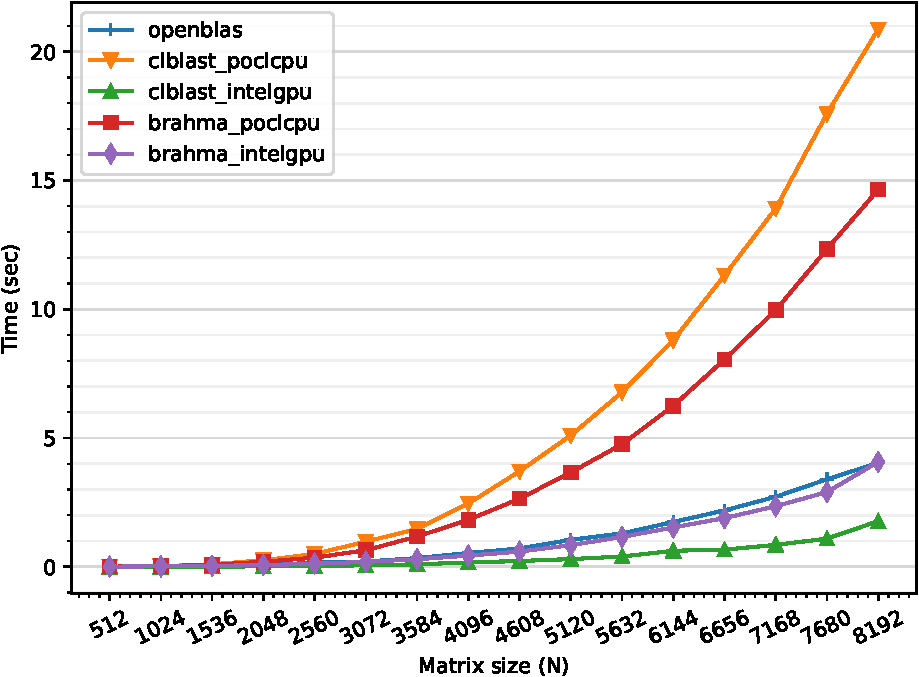
\includegraphics[width=0.45\textwidth]{../data/zenbook_iris_crop.pdf}
  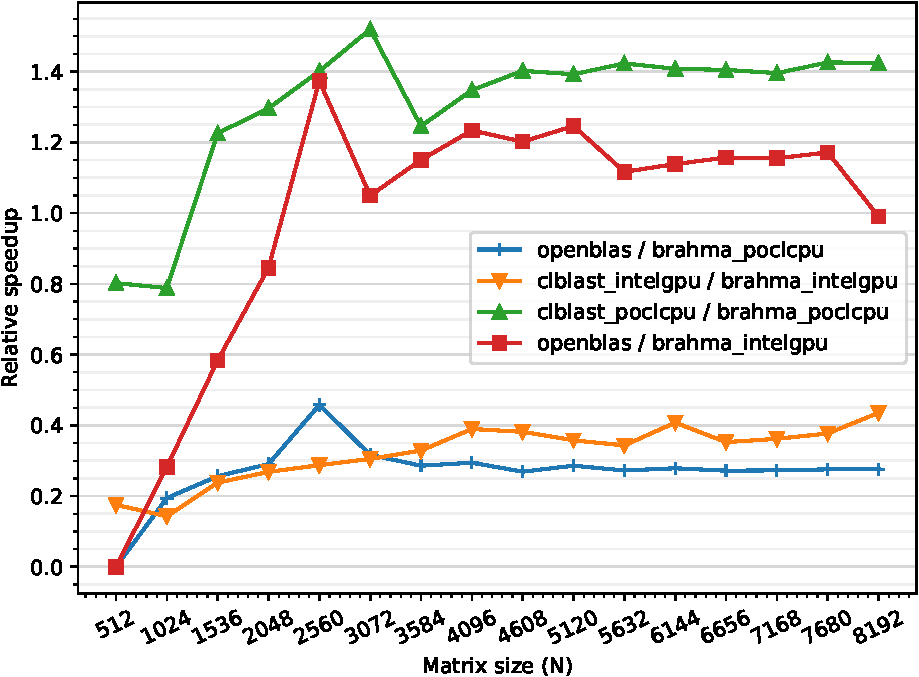
\includegraphics[width=0.45\textwidth]{../data/zenbook_iris_rel_crop.pdf}\\
  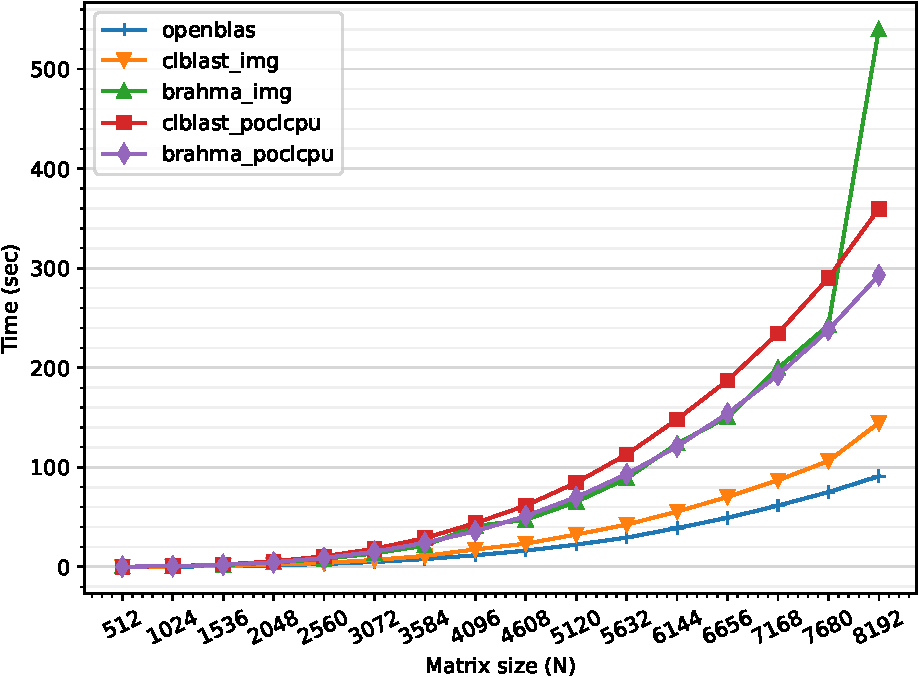
\includegraphics[width=0.45\textwidth]{../data/MILK-V_crop.pdf}
  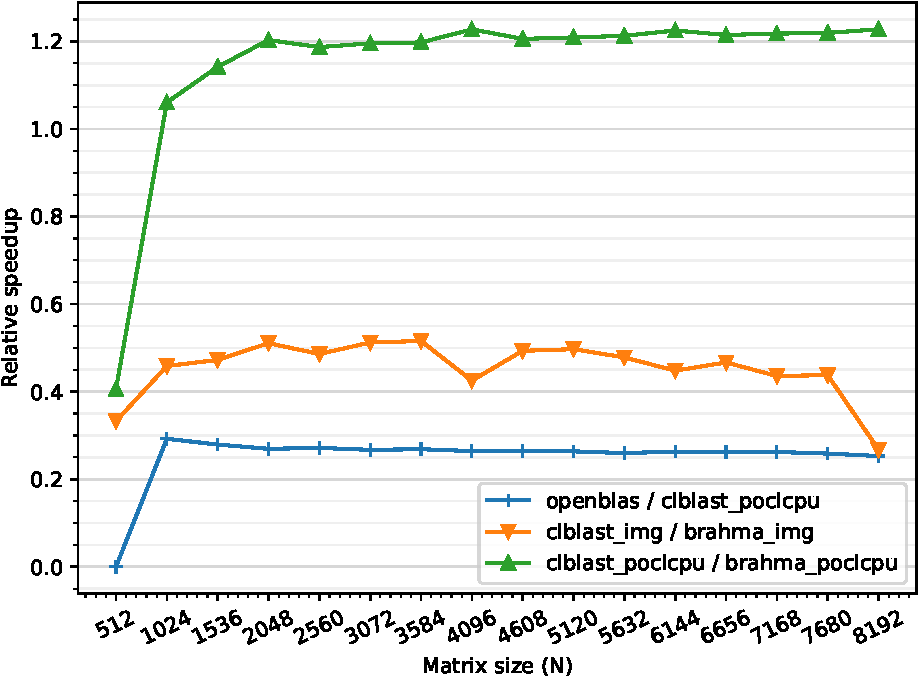
\includegraphics[width=0.45\textwidth]{../data/MILK-V_rel_crop.pdf}
  \end{center}
  \caption{Matrix multiplication performance: 1st row for \textbf{Lenovo}, 2nd for \textbf{Zen}, 3rd for \textbf{MILK-V}}
  \label{fig:mxm_perf}
\end{figure}

We choose two competitors.
The first one is the CLBlast\footnote{CLBlast source code: \url{https://github.com/CNugteren/CLBlast}}~\cite{10.1145/3204919.3204924} that is a highly-tuned (even for liw-power mobile GPUPUs) OpenCL-based BLAS implementation.
The second oe is the OpenBLAS\footnote{OpenBALAS source code: \url{https://github.com/OpenMathLib/OpenBLAS}} that is a highly-tuned BLAS implementation foe CPU.
All competitors were compiled and run with default settings.
Additionally, we run OpenCL-based solutions on CPUs using POCL~\cite{Jskelinen2014}.

We evaluate all competitors on several platforms listed below.
\begin{itemize}
  \item \textbf{Lenovo}: Intel Core i7-8550U CPU, NVIDIA GeForce MX150 and Intel(R) UHD Graphics 620 GPUs.
  \item \textbf{Zen}: Intel Core i5-1340P CPU, Intel Iris Xe Graphics G7 80EUs GPU.
  \item \textbf{MILC-V}. SpacemiT M1 CPU, IMG BXE-2-32 GPU.
  %\item \textbf{OrangePi}, Mali, ARM
\end{itemize}

We generate random square matrices with elements of type \texttt{float32} and use typical arithmetic semiring because our competitors does not provide generic kernels.
Time is measured as an average of 10 runs.
We measure time of client function execution, so it includes datatransfer.
Results of evaluation represented in figure~\ref{fig:mxm_perf}: we show both time and relative speedup.

First of all, we show that Brahma.FSharp allows one to create portable solutions.
Obviously, our kernel is not such optimized as kernel from CLBlast, but relative speedup analysis shows that more tuning required: in much cases performance gap decreases with data size increase (\textbf{Lenovo} esp. Intel GPU; \textbf{Zen}).
But in some cases behavior is more complex: for \textbf{MILC-V} our solution on CPU using POCL demonstrates better performance that CLBlast, but on respective GPU performance gap slightly increases with data size increase.

Such behavior can be explained by differences in kernel tuning, but not by technology problem.
So, while it is unlikely possible to hide dotnet overhead fully, it looks possible to minimize it to be comparable on big matrices.
To do it we should to create finer tuned and more flexible kernel to allows one better fit performance-affecting parameters.
\section{Conclusion and Future Work}

Brahma.FSharp---a tool for developing cross-platform, GPGPU-accelerated .NET applications---is presented.
We demonstrated applications portability by evaluating performance across multiple platforms, including RISC-V with PowerVR GPGPU and embedded Intel GPUs.

While the work remains in progress, Brahma.FSharp already enables creation of linear algebra kernels sufficiently performant for integration into libraries like Math.NET Numerics, allowing transparent offloading of generic linear algebra operations to GPGPUs.
Such integration is planned for the near future.

%Also, within the translator improvements, it is necessary to improve performance of data transferring between managed and native memory for complex types such as discriminated unions.
%For translator improvements, optimizing data transfer performance between managed and native memory for complex types (e.g., discriminated unions) requires further development.

Although the agent-based communication approach aligns naturally with both OpenCL and F\#, MailboxProcessor may not be optimal for high-frequency CPU-GPU communication.
Alternative solutions like Hopac\footnote{Hopac and MailboxProcessor performance comparison: \url{https://vasily-kirichenko.github.io/fsharpblog/actors}} or lightweight command queue wrappers could provide better performance for latency-critical code.

A significant challenge for future research involves automatic memory management.
Currently, GPGPU memory requires manual cleanup despite .NET's garbage collector.
Developing a hybrid approach that leverages automatic garbage collection while retaining manual control when needed remains an open problem.

%\section*{Acknowledgments}

We sincerely thank the anonymous reviewers for their thorough evaluation, insightful comments, and valuable suggestions that helped improve this work.
This research has been supported by the St. Petersburg State University, grant id 116636233.

\bibliographystyle{abbrv}
\bibliography{sigproc}

\end{document}